\chapter*{异常处理}
\label{chp:Java-exception-handling}

\section*{基本信息}
\sline
\begin{description}
\item[课程名称:] Java应用与开发
\item[授课教师:] 王晓东
\item[授课时间:] 第七周
\item[参考教材:] 本课程参考教材及资料如下:
  \begin{itemize}
  \item 陈国君主编,Java程序设计基础(第5版),清华大学出版社,2015.5
  \item Bruce Eckel, Thinking in Java (3rd)
  \end{itemize}
\end{description}

\section*{教学目标}

\sline

\begin{enumerate}
\item 掌握Java异常的概念和分类
\item 深入理解Java异常处理机制
\end{enumerate}  

\section*{授课方式}

\sline
\begin{description}
\item[理论课:] 多媒体教学、程序演示
\item[实验课:] 上机编程
\end{description}

\newpage
\section*{教学内容}
\sline

%%%%%%%%%%%%%%%%%%%%%%%%%%%%%%%%%%%%%%%%%%%%%%%%%%%%%%%%%%%%%%
\section{异常的概念及分类}

\subsection{什么是异常}

在Java语言中,程序运行出错被称为出现异常。异常(Exception)是程序运行过
程中发生的事件,该事件可以中断程序指令的正常执行流程。Java异常分为两大类:

\begin{description}
\item[错误(Error)] 是指JVM系统内部错误、资源耗尽等严重情况。
\item[违例(Exception)] 则是指其他因编程错误或偶然的外在因素导致的一般
  性问题,例如对负数开平方根、空指针访问、试图读取不存在的文件以及网络
  连接中断等。
\end{description}

给出一个Java运行时异常的示例:

\samplecode{TestException.java}

\begin{javaCode}
public class TestException {
  public static void main(String[] args) {
    String friends[] = {"Lisa", "Bily", "Kessy"};
    for(int i = 0; i < 5; i++) {
      System.out.println(friends[i]);
    }
    System.out.println("\n this is the end");
  }
}
\end{javaCode}

标准输出如下,程序编译通过,但运行时出错。

\begin{stdoutCode}
Lisa
Bily
Kessy
Exception in thread "main" java.lang.
ArrayIndexOutOfBoundsException: 3
at TestException.main(TestException.java:6)
\end{stdoutCode}

\subsection{Java异常分类}
 
Throwable类是Java语言中所有异常类的父类。Java异常分类如
图\ref{fig:exception-class}所示。

\begin{figure}[h]
\centering
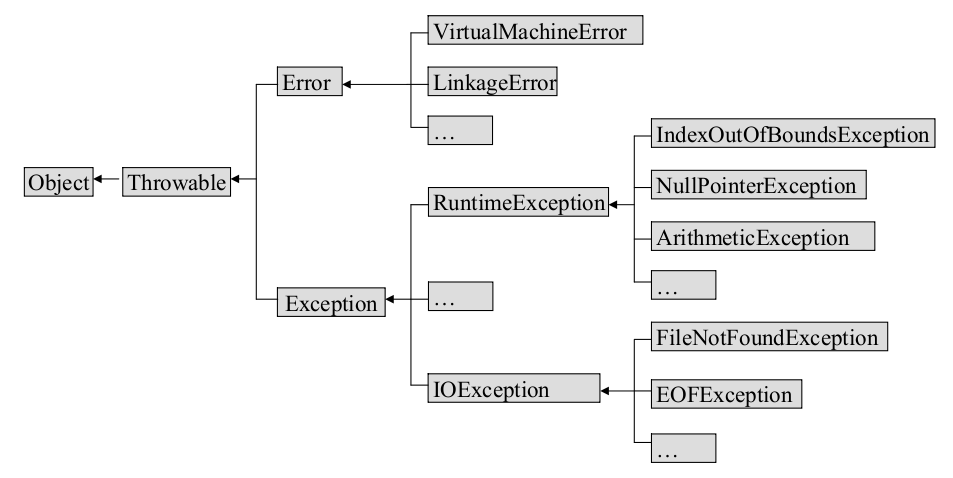
\includegraphics[width=0.95\textwidth]{images/Java-exception-handling/fig-exception-class.png}
\caption{Java异常分类}
\label{fig:exception-class}
\end{figure}

\subsection{常见错误}

\subsubsection{链接错误(LinkageError)}

LinkageError是指程序链接错误。例如,一个类中用到另外一个类,在编译前一
个类之后,后一个类发生了不相容的改变时,再使用前一个类则会出现链接错误。
最常见的就是后一个类的.class文件被误删除。

\subsubsection{虚拟机错误(VirtualMachineError)}
 
当Java虚拟机崩溃或用尽了它继续操作所需的资源时,会抛出该错误。其中比较
有代表性的是StackOverflowError,当应用程序递归太深而导致栈内存溢出时会
出现该异常。

\samplecode{TestVMerror.java}

\begin{javaCode}
  public class TestVMError {
    public static void main(String[] args) {
      TestVMError t = new TestVMError();
      t.f(100000);
    }
    public int f(int n) {
      if (n <= 0) {
        return 0;
      }
      int k = n * this.f(n-1);
      return k;
    }
  }
\end{javaCode}

标准输出如下:

\begin{stdoutCode}
  Exception in thread "main" java.lang.StackOverflowError
  at TestException.f(TestException.java:7)
  at TestException.f(TestException.java:10)  
\end{stdoutCode}

\subsection{常见异常}

\subsubsection{运行时异常(RuntimeException)}

运行时异常主要包括:

\begin{itemize}
\item 错误的类型转换;
\item 数组下标越;
\item 空指针访问。
\end{itemize}

其中,空指针异常(NullPointerException)是如果试图访问不指向任何对象的
引用变量的成员,将会产生空指针异常。例如:

\begin{javaCode}
Person p = null;
System.out.println(p.age);  
\end{javaCode}

\subsubsection{IO异常(IOException)}

\begin{itemize}
\item 从一个不存在的文件中读取数据;
\item 越过文件结尾继续读取;
\item 连接一个不存在的URL。
\end{itemize}

以下给出IOException的一个示例,注意下述代码无法通过编译!

\samplecode{TestIOException.java}

\begin{javaCode}
import java.io.*;
public class TestIOException {
  public static void main(String[] args) {
    FileInputStream in = new FileInputStream("myfile.txt");
    int b;
    b = in.read();
    while (b != -1) {
      System.out.print((char) b);
      b = in.read();
    }
    in.close();
  }
}  
\end{javaCode}

\notice{对上述代码无法编译的解释}

只要是有可能出现IOException的Java代码,在编译时就会出错,而不会等到运行
时才发生。编译出错信息大致如下:

\begin{stdoutCode}
TestIOException.java:4: 未报告的异常 java.io.FileNotFoundException; 
必须对其进行捕捉或声明以便抛出
    FileInputStream in = new FileInputStream("myfile.txt");
... ...
\end{stdoutCode}

\section{Java异常处理机制}

Java异常处理的宗旨包括:

\begin{itemize}
\item 返回到一个安全和已知的状态;
\item 能够使用户执行其他的命令;
\item 如果可能,则保存所有的工作;
\item 如果有必要,可以退出以避免造成进一步的危害。
\end{itemize}

Java异常处理的基本机制是:

\begin{itemize}
\item Java程序执行过程中如出现异常,系统会监测到并自动生成一个相应的异常类对象,然后再将它
  交给运行时系统;
\item 运行时系统再寻找相应的代码来处理这一异常。如果Java运行时系统找不到可以处理异常的代
  码,则运行时系统将终止,相应的Java程序也将退出。
\item 程序本身通常对错误(Error)无能为力,因而一般只处理违例(Exception)。
\end{itemize}

\subsection{捕获异常}

Java语言捕获异常的基本程序逻辑结构如下:

\begin{javaCode}
try {
  ... //可能产生异常的代码
} catch (ExceptionName1 e) {
  ... //当产生 ExceptionName1 型异常时的处置措施
} catch (ExceptionName2 e) {
  ... //当产生 ExceptionName2 型异常时的处置措施
} finally {
  ... //无条件执行的语句
}
\end{javaCode}

以下给出一段捕获处理数组访问越界异常的示例:

\samplecode{ArrayIndexOutOfBoundsExceptionSample.java}

\begin{javaCode}
public class ArrayIndexOutOfBoundsExceptionSample {
  public static void main(String[] args) {
    String friends[]={"Lisa","Billy","Kessy"};
    try {
      for(int i = 0; i < 5; i++) {
        System.out.println(friends[i]);
      }
    } catch(ArrayIndexOutOfBoundsException e) {
      System.out.println("index err");
    }
    System.out.println("\nthis is the end");
  }
}
\end{javaCode}

\subsection{使用finally语句}

Java异常处理中,finally语句是可选的,其作用是为异常处理提供一个统一的出口,使得在控制流转到程序的其他部分以前,能够对程序的状态作统一的管理。

\samplecode{FinallySample.java}

\begin{javaCode}
public class FinallySample {
  public static void main(String[] args) {
    String friends[]={"Lisa","Billy","Kessy"};
    try {
      for (int i = 0; i < 5; i++) {
        System.out.println(friends[i]);
      }
    } catch(ArrayIndexOutOfBoundsException e) {
      System.out.println("index err");
      return;
    } finally {
      System.out.println("in finally block!");
    }
    System.out.println("this is the end");
  }
}
  
\end{javaCode}

注意,不论try代码块中是否发生了异常事件,finally块中的语句都会被执行。当catch语句块中出现return
语句时,finally语句块同样会执行。上述代码的输出:

\begin{stdoutCode}
Lisa
Billy
Kessy
index err
in finally block!  
\end{stdoutCode}

\subsection{操纵异常对象}

发生异常时,系统将自动创建异常类对象,并将作为实参传递给匹配的catch语句块的形参,这样我们
就可以在语句块中操纵该异常对象了。主要使用异常类的父类Throwable中定义的两个成员方法:

\begin{itemize}
\item public String getMessage() 返回描述当前异常的详细消息字符串;
\item public void printStackTrace() 用来跟踪异常事件发生时运行栈的内容,并将相关信息输出
  到标准错误输出设备。本方法比较常用,在没有找到适合的异常处理代码时,系统也会自动调用该
  方法输出错误信息。
\end{itemize}

可以参考以下代码追踪运行栈信息:

\samplecode{A.java}

\begin{javaCode}
public class A {
  public void work(int[] a) {
    String s = this.contain(a, 3);
    System.out.println("Result: " + s);
  }

  public String contain(int[] source, int dest) {
    String result = "no!";
    try {
      for (int i = 0; i < source.length; i++) {
        if (source[i] == dest)
        result = "yes!";
      }
    } catch(Exception e) {
      System.out.println("异常信息:" + e.getMessage());
      System.out.println("运行栈信息:");
      e.printStackTrace();
      result = "error!";
    }
    return result;
  }
}
\end{javaCode}

\samplecode{MyTest.java}

\begin{javaCode}
public class MyTest {
  public static void main(String[] args) {
    A tst = new A();
    tst.work(null);
  }
}
\end{javaCode}

程序输出结果如下:

\begin{stdoutCode}
Exception Message: null
Stack Trace:
java.lang.NullPointerException
    at A.contain(A.java:9)
    at A.work(A.java:3)
    at MyTest.main(MyTest.java:4)
Result: error!
\end{stdoutCode}

\subsection{捕获和处理IOException}

以下给出捕获和处理IOException的示例:

\samplecode{TestIOException.java}

\begin{javaCode}
import java.io.*;
public class TestIOException {
  public static void main(String[] args) {
    try {
      FileInputStream in = new FileInputStream("myfile.txt");
      int b;
      b = in.read();
      while(b != -1) {
        System.out.print((char) b);
        b = in.read();
      }
      in.close();
    } catch (FileNotFoundException e) {
      System.out.println("File is missing!");
    } catch (IOException e) {
      e.printStackTrace();
    }
    System.out.println("It's ok!");
  }
}
\end{javaCode}

FileNotFoundException是IOException的子类,基于多态性机制,后一个catch语
句也可以处理FileNotFoundException,因此前一个catch语句块可以取消,但这
样就无法区分是“文件不存在”引发异常或其他I/O异常了。

\notice{异常处理知识点}

\begin{enumerate}
\item 对于只可能产生RuntimeException的代码可以不使用try-catch语句进行处
  理,如果对于这些相对安全的代码仍然采用了try语句块的形式,则try后可以
  省略catch语句块或finally语句块,但不能同时省略。
\item 如果试图捕获和处理代码中根本不可能出现的异常,编译器也会指出这种
  不当行为。
\end{enumerate}

\subsection{声明抛出异常}
 
声明抛弃异常是Java中处理违例的第二种方式如果。一个方法中的代码在运行时
可能生成某种异常,但在本方法中不必、或者不能确定如何处理此类异常时,则
可以声明抛弃该异常;此时方法中将不对此类异常进行处理,而是由该方法的调用
者负责处理。 语法格式如下:

\begin{javaCode}
  [< 修饰符 >] < 返回值类型 > < 方法名 > (< 参数列表 >) [throws < 异常类型 > [,< 异常类型 >]*] {
    [< Java语句 >]*
  }
\end{javaCode}

\samplecode{TestThrowsException.java}

\begin{javaCode}
import java.io.*;
public class TestThrowsException {
  public static void main(String[] args) {
    TestThrowsException t = new TestThrowsException();
    try {
      t.readFile();
    } catch (IOException e) {
      System.out.println(e);
    }
  }
  public void readFile() throws IOException {
    FileInputStream in = new FileInputStream("myfile.txt");
    int b;
    b = in.read();
    while (b != -1) {
      System.out.print((char) b);
      b = in.read();
    }
    in.close();
  }
}
\end{javaCode}
 
\notice{声明抛出异常的注意事项}

\begin{enumerate}
\item 除非事先约定,否则在开发过程中不要在自己编写的方法中采用抛出异常
  的方式。
\item 重写方法不允许抛出比被重写方法范围更大的异常类型。例
  如 IOException重写后抛出FileNotFoundException和EOFException被允许,而
  抛出Exception则不被允许。
\end{enumerate}
 
\subsection{人工抛出异常}

Java异常类对象除了在程序运行出错时由系统自动生成并抛出之外,也可根据需
要人工创建并抛出:

\begin{javaCode}
IOException e = new IOException(); // 创建异常类对象
throw e; // 抛出操作,即将该异常对象提交给Java运行环境
\end{javaCode}

被抛出的必须是Throwable或其子类类型的对象。例如,下述语句因为人工抛出的
并非Throwable或其子类的对象,在编译时会产生语法错误:

\begin{javaCode}
throw new String("want to throw");  
\end{javaCode}

以下给出一个人工抛出异常的示例:

\samplecode{TextThrowException.java}

\begin{javaCode}
import java.util.Scanner;

public class TestThrowException {
  public static void main(String[] args) {
    TestThrowException t = new TestThrowException();
    System.out.print("Please input your age: ");
    System.out.print("Your age: " + t.inputAge());
  }
  public int inputAge() {
    int result = -1;
    Scanner scan = new Scanner(System.in);
    while (true) {
      try {
        result = scan.nextInt();
        if (result < 0 || result > 130) {
          Exception me = new Exception("You come from Mars? ");
          throw me;
        }
        break;
      } catch (Exception e1) {
        System.out.println(e1.getMessage() + "Please input your age again: ");
        continue;
      }
    }
    return result;
  }
}
\end{javaCode}

上述代码所述的情况利用异常处理机制实现数据取值范围的检查并不太合适。应
用异常处理机制的原则如下:

\begin{itemize}
\item 当明确知道可能出错的地方或能够通过简单的检查而有效防止错误发生,
  就应该使用if-else语句来预防错误发生;
\item 只有当我们无法明确知道错误发生之处或无法完全避免异常,才不得不通
  过异常处理的方式来捕获和处理异常。
\end{itemize}


\section{用户自定义异常}

Java语言及许多类库针对常见异常状况已事先定义了相应的异常类型,并在程序
运行出错时由系统自动创建相应异常对象并进行抛出、捕获和处理,因此一般不
需要用户人工抛出异常对象或定义新的异常类型,但针对特殊的需要也可以这样
做。

我们一般通过继承Exception类来实现异常类型自定义,由于用户自定义的异常不
会由系统自动检测并抛出,所以只能靠人工触发并抛出。

以下给出用户自定义异常的示例:

\samplecode{CustomizingException.java}

\begin{javaCode}
public class CustomizingException extends Exception {
  private int idnumber;

  public MyException(String message, int id) {
    super(message);
    this.idnumber = id;
  }

  public int getId() {
    return idnumber;
  }
}
\end{javaCode} 

上述自定义异常类代码的构造方法中使用super调用其父类Exception的有参构造
方法,以便在创建异常对象时将用户的定制的报错信息传递给父类中定义
的private属性Message(该属性由Throwable类定义),将来在捕获和处理异常时
就可以通过调用该对象的getMessage()方法访问到该信息。

\samplecode{TestCustomizingException.java}

\begin{javaCode}
public class TestCustomizingException {
  public void regist(int num) throws MyException {
    if (num < 0) {
      throw new MyException("人数为负值,不合理", 3);
    }
    System.out.println("登记人数:" + num);
  }

  public void manager() {
    try {
      regist(-100);
    } catch (MyException e) {
      System.out.println("登记失败,出错种类" + e.getId());
      e.printStackTrace();
    }
    System.out.print("本次登记操作结束");
  }

  public static void main(String args[]) {
    new TestCustomizingException().manager();
  }
}
\end{javaCode}

上述测试程序输出结果如下:

\begin{stdoutCode}
登记失败,出错种类3
MyException: 人数为负值,不合理 ...
\end{stdoutCode}

\section{断言}

\subsection{什么是断言}

从JDK1.4版本开始,Java语言中引入了断言(Assert)机制,允许Java开发者在
代码中加入一些检查语句,主要目的是用于程序调试。

\begin{itemize}
\item 当我们需要在约定的条件不成立时中断当前程序执行操作的话可以使用断言;
\item 使用断言是为了在测试阶段确定程序内部出错位置和出错信息,而不是控制程序流程;
\item 断言机制在用户定义的boolean表达式(判定条件)结果为false时抛出一
  个Error对象,其类型为AssertionError;
\item 作为Error的一种,断言失败也不需捕获处理或者声明抛出,一旦出现了则
  终止程序、不必进行补救和恢复。

\end{itemize}

\subsection{启用和禁用断言}

\subsubsection{命令行开启断言功能}

Java运行时环境默认设置为关闭断言功能,因此在使用断言以前,需要在运
行Java程序时先开启断言功能。方法如下:

\begin{shCode}
>java -ea MyAppClass
\end{shCode}

或者:

\begin{shCode}
>java -enableassertions MyAppClass  
\end{shCode}

\subsubsection{命令行关闭断言功能}

\begin{shCode}
>java -da MyAppClass  
\end{shCode}

或者:

\begin{shCode}
java -disableassertions MyAppClass  
\end{shCode}

\subsubsection{Eclipse IDE开启断言}

在项目上点击右键 \ding{224} Run As \ding{224} Run Configurations \ding{224} Arguments,
在VM arguments中,加入-enableassertions或-ea即可。

\subsection{使用断言}

第一种断言的语法格式如下:

\begin{javaCode}
assert <boolean 表达式>;  
\end{javaCode}

以下给出使用第一种断言语法的示例代码:

\samplecode{TestAssertion.java}

\begin{javaCode}
public class TestAssertion {
  public static void main(String[] args) {
    new TestAssertion().process(-12);
  }
  public void process(int age) {
    assert age >= 0;
    System.out.println("您的年龄:" + age);
    // ---
  }
}
\end{javaCode}

以上程序执行的输出如下:

\begin{stdoutCode}
Exception in thread "main" java.lang.AssertionError
	at TestAssertion.process(TestAssertion.java:8)
	at TestAssertion.main(TestAssertion.java:4)  
\end{stdoutCode}

第二种断言的语法格式如下:

\begin{javaCode}
assert < boolean 表达式 >:< 表达式 2 >;  
\end{javaCode}

以下给出第二种断言格式的示例代码:

\samplecode{TestAssertion2.java}

\begin{javaCode}
public class TestAssertion2 {
  public static void main(String[] args) {
    new TestAssertion2().process(-12);
  }
  public void process(int age) {
    assert age >= 0: "年龄值不合理";
    System.out.println("您的年龄:" + age);
    //---
  }
}
\end{javaCode}

输出结果如下:

\begin{stdoutCode}
Exception in thread "main" java.lang.AssertionError: 年龄值不合理
	at TestAssertion.process(TestAssertion.java:8)
	at TestAssertion.main(TestAssertion.java:4)  
\end{stdoutCode}

\descript{说明}

断言失败时,系统会自动将表达式2的值传递给新创建的AssertionError对象,进
而将其转换为一个消息字符串保存起来,这样就可以在获得更多/更有针对性的检
查失败细节信息。因此,其中的表达式2可以是任何基本数据类型或引用数据类型,
但必须提供一个值,即不能为空值。

